\chapter{MARCO TEÓRICO}\label{sec:theorethical_framework}

%\section{Theorethical Framework}%\label{sec:theorethical_framework}
Éste capítulo presenta una introducción a los conceptos principales utilizados en éste trabajo. Solamente se busca presentar los conceptos fundamentales, necesarios para comprender los detalles técnicos del mismo.

Primeramente se muestran conceptos relacionados al procesamiento de la imagen, y luego se enfoca en los conceptos fundamentales necesarios para comprender la metaheurística asociada.
%This sections presents a brief introduction of the concepts used in the paper.
%The solution proposed in this paper is based in the following concepts, which are to be described briefly below. It is fundamental to explain the color spaces, the meta-heuristic and the metrics adopted in this approach.

\section{Ecualización del Histograma}

La Ecualización del Histograma es un método de transformación de los pixeles de la imagen digital, cuya finalidad es ajustar el contraste de la misma. En general, la implementación básica de la Ecualización del Histograma toma todos los pixeles de la imagen, realiza una transformación del histograma de intensidades, e incrementa el contraste global de manera a tener una mejor distribución de intensidades dentro de la imagen. Una ventaja importante de esta técnica es que es una transformación directa y además un operador invertible; además los cálculos necesarios no son intensivos en el sentido computacional.

Existen modificaciones de la técnica básica, que abordan el problema utilizando múltiples histogramas (llamados subhistogramas), cuyo efecto importante es que logran mejoras en el contraste a nivel local. Los ejemplos más importantes son \textit{Adaptive Histogram Equalization} \cite{pizer1987adaptive}, \textit{Contrast Limited Adaptive Histogram Equalization} \cite{zuiderveld1994contrast}, MultiPeak Histogram Equalization (MPHE) \cite{743808}, y \textit{Multipurpose Beta Optimized Bihistogram Equalization (MBOBHE)}. Con éstos algoritmos se busca principalmente la mejora en el contraste sin que ocurra desplazamiento en el brillo medio o artefactos que produzcan pérdidas en detalles a consecuencia de las transformaciones ocurridas.

\subsection{Implementación Básica}

Si se considera una imagen digital discreta en escala de grises $I$, sea la probabilidad de ocurrencia de un nivel de gris $r_k$ dentro de la imagen una aproximación de la forma:

\begin{equation}
p_r(r_k)= \frac{n_k}{n} \qquad k=0,1,2,...,L-1
\end{equation}

donde $n$ es es el número total de pixeles de la imagen, $n_k$ es el número de pixeles que poseen el nivel de gris $r_k$, y $L$ es número de pixeles representables en la imagen. Se busca una función de transformación de los niveles de intensidad de los pixeles de la forma:

\begin{equation}
\begin{split}
s_k=T(r_k) & = \sum_{j=0}^k p_r(r_j) \\
& = \sum_{j=0}^k \frac{n_j}{n} \qquad k=0,1,2,...,L-1
\end{split}
\label{eq:ecualizacionhistograma}
\end{equation}

Entonces, una imagen resultante se obtiene a partir del mapeo de cada pixel de nivel de intensidad $r_k$ de la imagen de entrada con un pixel correspondiente de nivel de intensidad $s_k$ utilizando la ecuación \ref{eq:ecualizacionhistograma}. 

\subsection{Ejemplo de aplicación}

Mediante un ejemplo es posible clarificar el concepto presentado arriba. Por lo tanto, si asumimos una imagen digital de 4096 pixeles con $L=8$ niveles de gris. La tabla siguiente muestra de manera resumida el proceso correspondiente a la ecualización del histograma básica:

\begin{table}[H]
\centering
\begin{tabular}{ ? r | r | c | c | c ?}
\hlineB{2}
\rowcolor{SeaGreen3!30!} $r_k$ & $n_i$ & $n_i/N$ & $cdf(r_k)$ & $s_k$ \\ \hlineB{2}
0 & 790  & 0,19 & 0,19 & $0,19 \times 7 \approx 1$ \\ \hline
1 & 1023 & 0,25 & 0,44 & $0,44 \times 7 \approx 3$ \\ \hline
2 & 850  & 0,21 & 0,65 & $0,65 \times 7 \approx 5$ \\ \hline
3 & 656  & 0,16 & 0,81 & $0,81 \times 7 \approx 6$ \\ \hline
4 & 329  & 0,08 & 0,89 & $0,89 \times 7 \approx 6$ \\ \hline
5 & 245  & 0,06 & 0,95 & $0,95 \times 7 \approx 7$ \\ \hline
6 & 122  & 0,03 & 0,98 & $0,98 \times 7 \approx 7$ \\ \hline
7 & 81   & 0,02 & 1,00 & $1,00 \times 7 = 7$ \\ \hlineB{2}
\end{tabular}
\caption{Proceso de ecualización de histograma básica. La columna $r_k$ representa los niveles de gris de la imagen original, y la columna $s_k$ muestra los niveles de gris que se mapean a partir del proceso, y que reemplazarán a los valores de $r_k$ en la imagen procesada.}
\label{tab:ejemploeqhistograma}
\end{table}

La Tabla \ref{tab:ejemploeqhistograma} muestra el proceso de ecualización de una imagen de ejemplo. Si se representa una imagen digital con 3 bits (lo cual permite representar 8 niveles de intensidad en la imagen digital), y se tiene el conteo de pixeles para cada nivel como se muestra en la columna $n_i$, entonces el proceso de normalización será como se ve en la columna $n_i/N$, el $CDF$ se calcula como se muestra en la columna $cdf(r_k)$ y finalmente el nivel de gris mapeado será el que se muestra en la columna $s_k$.

% \begin{figure}[H]
%     \centering
%     %\begin{subfigure}[t]{0.45\textwidth}
%     \begin{subfigure}[]{
%         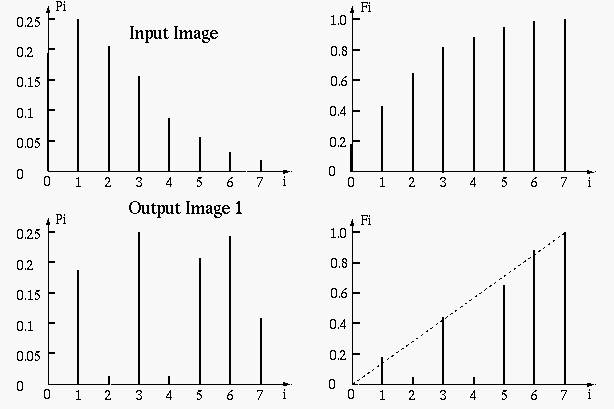
\includegraphics[width=0.50\textwidth]{./Figures/equalize2.jpg}
%     }
% %        \caption{Imagen Original. $\mathscr{H_Y}=0.207231$, $SSIM_R=1$, $SSIM_G=1$, $SSIM_B=1$}
% %        \label{fig:cuborgb}
%     \end{subfigure}
%     \caption{Histograma y $CDF$ de la imagen Original. Abajo, Histograma y $CDF$ de la imagen ecualizada.}\label{fig:ejemploeqhistograma2}
% \end{figure}

\begin{figure}[H]
\centering
\begin{subfigure}[]{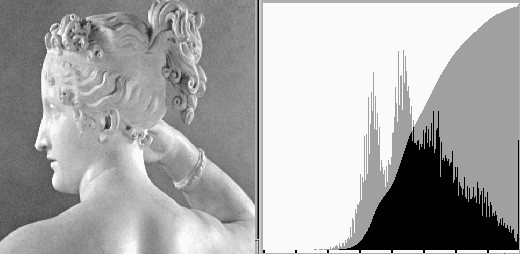
\includegraphics[width=\textwidth]{./Figures/Paolina_256_hist.jpg}}
\caption{Imagen original (sin procesar) y su correspondiente histograma y $CDF$}
\label{fig:ejemploeqhistograma3}
\end{subfigure} 

    ~ %add desired spacing between images, e. g. ~, \quad, \qquad, \hfill etc. 
    %(or a blank line to force the subfigure onto a new line)
    \begin{subfigure}[]{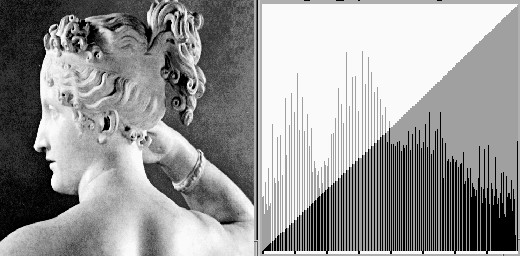
\includegraphics[width=\textwidth]{./Figures/Paolina_256_hist_eq.jpg}}
    \caption{Imagen con contraste mejorado (luego de la aplicación de la ecualización del histograma) con su correspondiente histograma y $CDF$}
    \label{fig:ejemploeqhistograma4}
    \end{subfigure}
    \caption{Imágenes original y resultante luego de la aplicación de la ecualización del histograma. A la izquierda de cada una se observa el histograma y el $CDF$ respectivo a cada imagen.}\label{fig:ejemplohistograma5}
    \end{figure}

% En la Tabla \ref{tab:ejemploeqhistograma} se muestra cuál es el proceso de mapeo de niveles de intensidad a partir de los niveles de gris $r_k$ de la imagen digital original, hasta los nuevos niveles de gris mapeados $s_k$. 

La Figura \ref{fig:ejemploeqhistograma3} muestra una imagen sin procesar, con su correspondiente histograma y $CDF$ previos al proceso de ecualización; en la Figura \ref{fig:ejemploeqhistograma4} se muestra la imagen obtenida luego de aplicar el proceso de ecualización, y los correspondientes histograma y $CDF$ resultantes luego de éste proceso. 

\section{Contrast Limited Adaptive Histogram Equalization (CLAHE)}\label{sec:clahe}

El algoritmo presentado en la sección anterior toma la imagen completa para realizar la tarea de ecualización del histograma. Ésto en general no es adecuado cuando se trabaja con imágenes cuyos detalles son cruciales para la posterior utilidad de la imagen transformada (imágenes aéreas, médicas, biométricas, y otras); es por éste motivo que se estudian (y en éste trabajo en particular se adoptan) algoritmos de mejora de contraste basados en ecualización del histograma por regiones, o algoritmos de ecualización locales.

En particular, Contrast Limited Adaptive Histogram Equalization (CLAHE) \cite{zuiderveld1994contrast} es un algoritmo bien conocido para la Mejora del Contraste, diseñado para ser aplicado de manera amplia en el contexto del procesamiento digital de imágenes. CLAHE es una variación del algoritmo de Mejora del Contraste denominado \textit{Adaptive Histogram Equalization (AHE)} \cite{pizer1987adaptive}. Ambas técnicas se explican en las subsecciones siguientes debido a la cercanía existente por la similaridad en cuanto a la implementación.

\subsection{Adaptive Histogram Equalization}\label{sec:definicionclahe}

El problema con la ecualización del histograma ordinaria, es que la imagen digital podría tener regines significativamente más oscuras o claras que el resto de la imagen, por lo que el contraste en esas regiones podría no mejorar significativamente.

En AHE, una imagen es procesada transformando cada pixel utilizando una función basada en el histograma de los pixeles que lo rodean; en principio éste algoritmo se desarrolló para su uso en displays de cabina de aviones de guerra \cite{ketcham1974image}. En su forma más simple, cada pixel se transforma en base al histograma de la región que envuelve al pixel. La derivación de las funciones de transformación de los histogramas locales es exactamente el mismo que en la ecualización del histograma ordinaria: La función de transformación es proporcional a la función de distribución acumulativa $CDF$ de los valores de pixeles de la vecindad. 

\subsubsection{Propiedades de AHE}

\begin{itemize}
    \item El tamaño de la región de vecindad es un parámetro del método. 
    \item Cuando una región de la imagen que contiene a un vecindario de pixeles es relativamente homogénea en cuanto a intensidades, el histograma resultante posee picos fuertes, y la función de transformación mapea un rango de intensidades corto a todo el rango de la imagen resultante. Ésto causa que $AHE$ amplifique porciones pequeñas de ruido en regiones de la imagen con intensidades homogéneas.
\end{itemize}

\subsection{Contrast Limited AHE}

Contrast Limited $AHE$ ($CLAHE$) es diferente a la ecualización adaptativa del histograma descrita arriba debido al esquema de limitación del contraste impuesto. $CLAHE$ se desarrolló para prevenir la sobre-amplificación de ruido que se percibe en $AHE$.

Éste problema se supera limitando la mejora del contraste realizada por $AHE$. La amplificación del contraste en la vecindad de un pixel de intensidad dada está relacionada a la pendiente de la función de transformación. Ésto significa que la amplificación es proporcional a la pendiente de la $CDF$ del vecindario y por tanto al valor del histograma a partir de ese valor de pixel. $CLAHE$ limita la amplificación recortando el histograma de acuerdo a un coeficiente predefinido, denominado \textit{Clip Limit} antes de computar el $CDF$. Ésto limita la pendiente del $CDF$ y por tanto la función de transformación.

Es importante no descartar la parte del histograma que excede a \textit{Clip Limit}\label{symbol:clahecliplimit} sino que se redistribuye de manera igualitaria entre todas las columnas del histograma, como se muestra en la Figura \ref{fig:redistclahe}.

\begin{figure}[H]
\centering
    %\begin{subfigure}[t]{0.45\textwidth}
    \begin{subfigure}[]{
    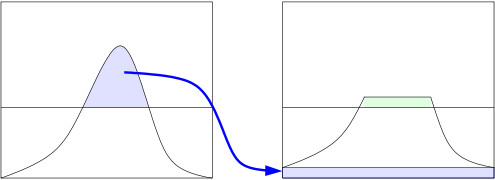
\includegraphics[width=0.50\textwidth]{./Figures/495px-Clahe-redist.jpg}
    }
%        \caption{Imagen Original. $\mathscr{H_Y}=0.207231$, $SSIM_R=1$, $SSIM_G=1$, $SSIM_B=1$}
%        \label{fig:cuborgb}
\end{subfigure}
\caption{Redistribución de niveles de intensidad dentro del histograma de una región de una imagen, como paso previo al cálculo del $CDF$. Ésto tiene como efecto la suaviación del proceso de mejora del contraste.}\label{fig:redistclahe}
\end{figure}


% Contrast Limited Adaptive Histogram Equalization (CLAHE) \cite{zuiderveld1994contrast} is a well known CE algorithm, designed for broad applicability in the context of digital image proccessing. CLAHE is a variation of the \textit{Adaptive Histogram Equalization (AHE)}\cite{pizer1987adaptive} CE algorithm. In AHE, an image is processed transforming each pixel using a function based on the histogram of its surrounding pixels, defined by a \textit{Contextual Region $(\mathscr{R}_x,\mathscr{R}_y)$}. CLAHE limits the CE by clipping the resultant histogram based in a coefficient called \textit{Clip Limit} $\mathscr{C}$

\section{Espacios de Color Adoptados}\label{sec:color_spaces}

Los Espacios de Color \cite{gonzalez02a} son representaciones de color de las imágenes digitales, que por lo general se aceptan mediante convención o por estándar de hecho. Por lo general, los Espacios de Color consisten en sistemas de coordenadas donde cada punto es un color representable dentro del Espacio.

En éste trabajo se utilizan dos espacios de color importantes dentro de la literatura, los cuales son analizados en las subsecciones siguientes: $RGB$ y $YCbCr$.

\subsection{El espacio de colores \textit{Red, Green, Blue}} 

El primer espacio importante a analizar en este trabajo es $RGB$ (del inglés $Red$, $Green$, $Blue$). $RGB$ es un modelo de color aditivo en el cual las luces de color $rojo$, $verde$, y $azul$ se agregan de varias maneras de forma a reproducir un conjunto amplio de clolores. El propósito principal de éste modelo es la percepción, representación y muestra de imágenes en sistemas electrónicos tales com televisores y computadoras, a pesar de que también se utilizó en la fotografía convencional.

En el modelo $RGB$, cada color aparece como un componente primario del $Rojo$, $Verde$ y $Azul$. Éste modelo sencillo se basa en el sistema de coordenadas Cartesianas. En la Figura \ref{fig:cuborgb} se pueden apreciar algunos colores notables representados en el espacio $RGB$: por ejemplo, el azul puro se representa como $(0,0,1)$, el verde puro como $(0,1,0)$ y el rojo puro como $(1,0,0)$; mientas que el negro se representa como $(0,0,0)$ y el blanco como $(1,1,1)$. Se puede apreciar la ventaja de usar ese sistema de representación de colores, el cual es sencillo. Se asume un sistema de coordenadas normalizado.

\begin{figure}[H]
\centering
    %\begin{subfigure}[t]{0.45\textwidth}
    \begin{subfigure}[]{
    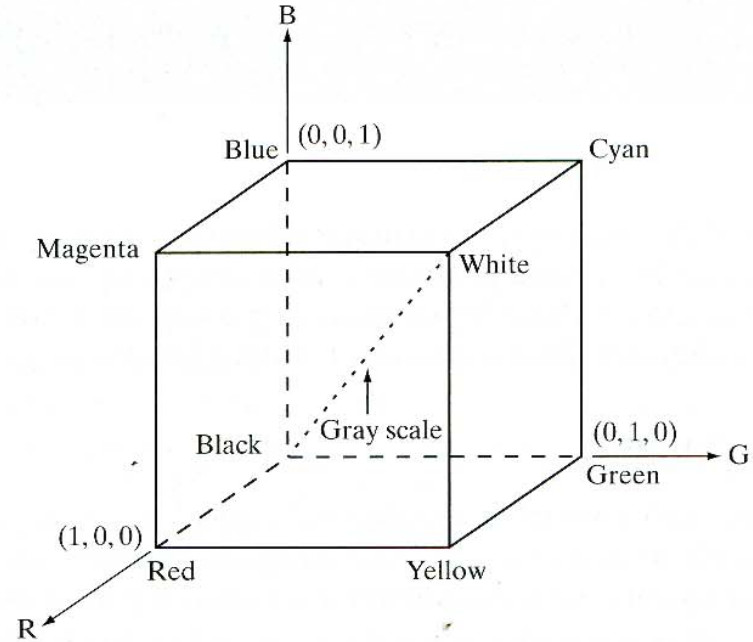
\includegraphics[width=0.50\textwidth]{./Figures/cubo-rgb.jpg}
    }
%        \caption{Imagen Original. $\mathscr{H_Y}=0.207231$, $SSIM_R=1$, $SSIM_G=1$, $SSIM_B=1$}
%        \label{fig:cuborgb}
\end{subfigure}
\caption{Diagrama esquemático del cubo que representa al espacio de colores $RGB$. Se pueden apreciar algunos colores notables.}\label{fig:cuborgb}
\end{figure}

En este trabajo, las imágenes originales se representan utilizando el espacio de colores $RGB$; en éste caso se tiene un arreglo de pixeles de color de tamaño $N \times M \times 3$. Cada pixel de color está representado por un elemento $[\begin{matrix}z_r & z_g & z_b\end{matrix}]$ del arreglo previamente mencionado, donde $z_r, z_g, z_b$ son los componentes rojo, verde y azul de un pixel de color en una ubicación específica. 

\subsection{El espacio de colores $YCbCr$}

Las imágenes originales son luego transformadas al espacio de colores $YCbCr$ \cite{gonzalez2002processing}, el cual es una representación ampliamente utilizada en el video digital. En esta representación $Y$ representa la información de luminancia de la imagen, mientras que el componente $Cb$ representa la diferencia entre el componente azul y un valor de referencia, mientras que el componente $Cr$ es la diferencia entre el componente rojo y un valor de referencia. Otra ventaja importante de ésta representación es que la conversión desde $RGB$, y nuevamente hacia $RGB$ es directa:

\begin{equation}
\begin{bmatrix}
Y \\
C_b \\
C_r 
\end{bmatrix} =
\begin{bmatrix}
16  \\
128 \\
128
\end{bmatrix}
+
\begin{bmatrix}
65.481 & 128.553 & 24.966 \\
-37.797 & -74.203 & 112.000 \\
112.000 & -93.786 & -18.214 
\end{bmatrix}
\begin{bmatrix}
R \\
G \\
B 
\end{bmatrix}
\end{equation}
\begin{equation}
\begin{bmatrix}
R \\
G \\
B 
\end{bmatrix} =
\begin{bmatrix}
Y + 1.402 \cdot (C_r - 128) \\
Y -0.34414 \cdot (C_b - 128) - 0.71414 \cdot (C_r - 128) \\
Y + 1.772 \cdot  (C_b - 128) 
\end{bmatrix}
\end{equation}

En la Figura \ref{fig:ejemploycbcr} se muestra cómo se separan los planos de $Y$ (intensidad) de los planos de color $Cb$ y $Cr$ respectivamente. Ésta separación pone en evidencia la conveniencia de ésta representación de colores, considerando que utilizar un canal de intensidades es adecuado para el algoritmo de mejora de contraste descripto en la Sección \ref{sec:clahe}.
\fboxrule=2pt
\begin{figure}[H]
\centering
    %\begin{subfigure}[t]{0.45\textwidth}
    % \begin{subfigure}[]{
    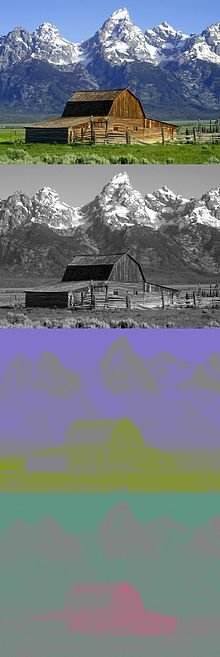
\includegraphics[width=0.50\textwidth, frame]{./Figures/220px-Barns_grand_tetons_YCbCr_separation.jpg}
    % }
%        \caption{Imagen Original. $\mathscr{H_Y}=0.207231$, $SSIM_R=1$, $SSIM_G=1$, $SSIM_B=1$}
%        \label{fig:cuborgb}
% \end{subfigure}
\caption{Imagen de ejemplo con las representaciones de intensidad ($Y$) y de color ($Cb,Cr$). Nótese que el mapa de intensidades $Y$ es una representación en escala de grises de la imagen digital.}\label{fig:ejemploycbcr}
\end{figure}

% Original images are represented using the $RGB$ color space \cite{gonzalez2002processing}, which is a $N \times M \times 3$  array of color pixels. Every color pixel is represented by an element $[\begin{matrix}z_r & z_g & z_b\end{matrix}]$ of the array previously mentioned, where $z_r, z_g, z_b$ are the red, green, and blue components of the color pixel in a specific location. Original images are then transformed to the $YCbCr$ color space \cite{gonzalez2002processing}, which is a representation widely used in digital video. The main advantage is that the $Y$ component here represents the luminance information of the image, meanwhile the $Cb$ component represents a difference between the blue component and a reference value, and the $Cr$ component is the difference between the red component and a reference value. Another important advantage of this representation is that the conversion from $RGB$, and back to $RGB$ is straightforward:



% \begin{equation}
% \begin{bmatrix}
%     Y \\
%     C_b \\
%     C_r 
% \end{bmatrix} =
%  \begin{bmatrix}
%     16  \\
%     128 \\
%     128
% \end{bmatrix}
% +
%  \begin{bmatrix}
%     65.481 & 128.553 & 24.966 \\
%     -37.797 & -74.203 & 112.000 \\
%     112.000 & -93.786 & -18.214 
% \end{bmatrix}
% \begin{bmatrix}
%    R \\
%    G \\
%    B 
% \end{bmatrix}
% \end{equation}
% \begin{equation}
% \begin{bmatrix}
%     R \\
%     G \\
%     B 
% \end{bmatrix} =
%  \begin{bmatrix}
%     Y + 1.402 \cdot (C_r - 128) \\
%     Y -0.34414 \cdot (C_b - 128) - 0.71414 \cdot (C_r - 128) \\
%     Y + 1.772 \cdot  (C_b - 128) 
% \end{bmatrix}
% \end{equation}



\section{Multi-Objective Particle Swarm Optimization (MOPSO)}

En este trabajo se aplica un enfoque Metaheurístico al problema de encontrar parámetros adecuados para el algoritmo de Mejora del Contraste, con miras a lograr una buena correlación entre objetivos de contraste y distorsión.


\textit{Particle Swarm Optimization (PSO)} es una Metaheurística computacional que optimiza un problema buscando mejorar soluciones candidatas de manera iterativa, moviendo las partículas dentro de un espacio de búsqueda definido por los parámetros de entrada del algoritmo sobre el que se aplica, y moviendo las partículas de acuerdo a fórmulas matemáticas simples de velocidad y posición. 

$PSO$ se atribuye originalmente a Kennedy, Eberhart y Shi \cite{488968,699146}

En la Figura \ref{fig:comportamientopso} se puede ver como unas soluciones candidatas se mueven dentro de un espacio de búsqueda, de manera de optimizar un objetivo.

En $PSO$, cada solución potencial del problema que se trata se denomina \textit{particle} y la población actual de soluciones se llama \textit{swarm}. Cada partícula $\vv{x}$\label{symbol:mopsoparticula} realiza una búsqueda dentro de un espacio de búsqueda $\Omega$, y para cada generación $t$, cada solución $\vv{x}$ se actualiza de acuerdo a: 


\begin{equation}\label{eq:posicion1}
\vv{x}_i(t) = \vv{x}_i(t-1) + \vv{v}_i(t)
\end{equation}

%Multi-Objective Particle Swarm Optimization ($MOPSO$) \cite{nebro2009smpso} is a widely known metaheuristic algorithm. It is a bio-inspired metaheuristic which mimics the social behavior of bird flocking. In $PSO$, every potential solution of the problem being approached is called a \textit{particle} and the actual population of solutions is called a \textit{swarm}. Every particle $\vv{x}$ performs a search within a search space $\Omega$, and for every generation $t$, every solution $\vv{x}$ is updated according to:

% \begin{equation}\label{eq:posicion1}
% \vv{x}_i(t) = \vv{x}_i(t-1) + \vv{v}_i(t)
% \end{equation}

Aquí, $\vv{v}$\label{symbol:mopsovelocidad} es un factor conocido como la velocidad, y está dado por:

\begin{equation}\label{eq:velocidad1}
\vv{v}_i(t) = w \cdot (t-1) + C_1 \cdot r_1 \cdot (\vv{x}_{p_i} - \vv{x}_i) + C_2 \cdot r_2 \cdot (\vv{x}_{g_i} - \vv{x_i}) \text{,}
\end{equation}

donde $\vv{x}_{p_i}$ es la mejor solución que $\vv{x}_i$ encontró hasta ahora, $\vv{x}_{g_i}$ es la mejor solución que el enjambre completo encontró durante una iteración, $w$ es un coeficiente conocido como el \textit{peso de la inercia}, que controla la tasa de velocidad de la búsquda de $PSO$; $r_1$ y $r_2$ son números aleatorios entre $[0,1]$. Finalmente, $C_1$ Y $C_2$ son los coeficientes que controlan la ponderación entre partículas globales y locales durante la búsqueda.


Multi-Objective Particle Swarm Optimization ($MOPSO$) \cite{nebro2009smpso} es la versión de $PSO$ para enfoques de optimización con más de un objetivo. Se añaden determinadas características para lograr cierta eficiencia durante el proceso de optimización definido arriba, y se basa en el concepto de \textit{Dominancia Pareto} para determinar las soluciones que se proponen como óptimas en el contexto de optimización Multi-Objetivo.

En $MOPSO$ se añaden algunas características a $PSO$, a saber: un \textit{coeficiente de constricción} $\chi$ se adopta de manera a controlar la velocidad de la partícula, como se describe abajo:

\begin{equation}
\chi = \frac{2}{2 - \varphi - \sqrt{\varphi^2 - 4 \varphi}}
\end{equation}

\begin{figure}[tbh]
\centering
    %\begin{subfigure}[t]{0.45\textwidth}
    \begin{subfigure}[]{
    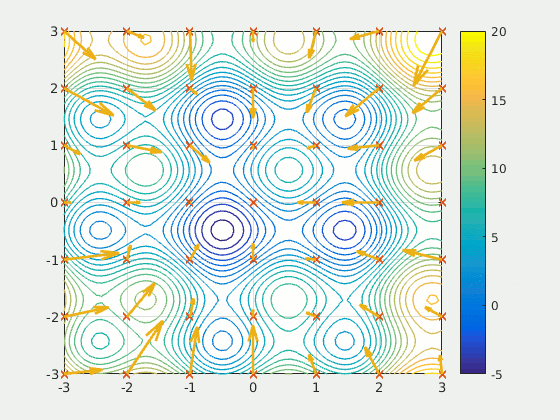
\includegraphics[width=0.45\textwidth]{./Figures/ejemplopso/capas-0.png}
    }
%        \caption{Imagen Original. $\mathscr{H_Y}=0.207231$. $SSIM_R=1$. $SSIM_G=1$. $SSIM_B=1$}
\end{subfigure}
    ~ %add desired spacing between images. e. g. ~. \quad. \qquad. \hfill etc. 
      %(or a blank line to force the subfigure onto a new line)
      \begin{subfigure}[]{
      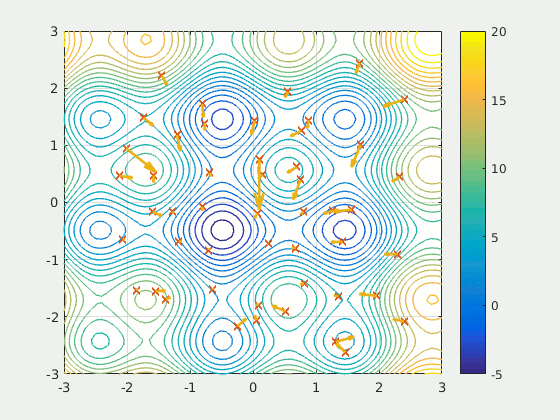
\includegraphics[width=0.45\textwidth]{./Figures/ejemplopso/capas-8.png}   
      }
    %\begin{subfigure}[t]{0.45\textwidth}
%        \caption{Enhanced Image. $\mathscr{H_Y}=0.611275$. $SSIM_R=0.00897331$. $SSIM_G=0.00823064$. $SSIM_B=0.00851013$}
\end{subfigure}
    ~ %add desired spacing between images. e. g. ~. \quad. \qquad. \hfill etc. 
    %(or a blank line to force the subfigure onto a new line)
    \begin{subfigure}[]{
    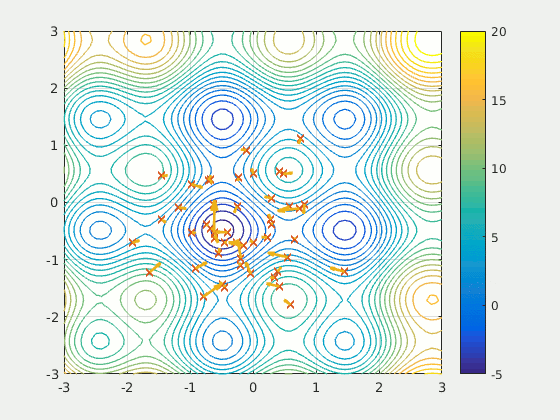
\includegraphics[width=0.45\textwidth]{./Figures/ejemplopso/capas-21.png}
    }
    % \begin{subfigure}[t]{0.45\textwidth}
%        \caption{Enhanced Image.  $\mathscr{H_Y}=0.0350595$. $SSIM_R=0.416776$. $SSIM_G=0.403636$. $SSIM_B=0.417654$}
\end{subfigure} 
\begin{subfigure}[]{
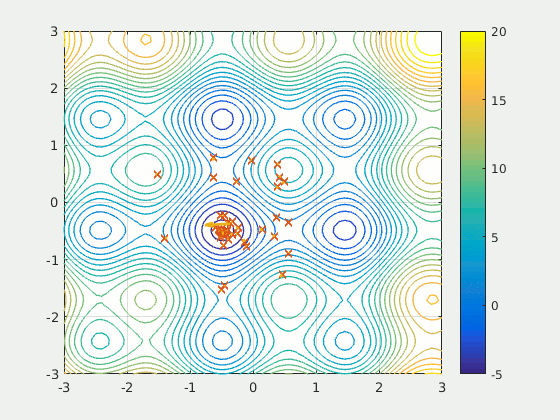
\includegraphics[width=0.45\textwidth]{./Figures/ejemplopso/capas-42.png}
}
    % \begin{subfigure}[t]{0.45\textwidth}
        %\caption{Enhanced Image using \cite{morepso}. $\mathscr{H_Y}=0.788927$. $SSIM_R=0.000204143$. $SSIM_G=0.0000526475$. $SSIM_B=0.0000518143$}
        \label{fig:calhouse23129}
        \end{subfigure}
    ~ %add desired spacing between images. e. g. ~. \quad. \qquad. \hfill etc. 
    %(or a blank line to force the subfigure onto a new line)
    \begin{subfigure}[]{
    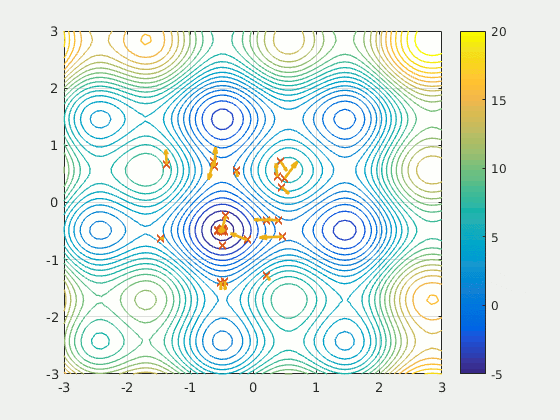
\includegraphics[width=0.45\textwidth]{./Figures/ejemplopso/capas-75.png}
    }
    % \begin{subfigure}[t]{0.45\textwidth}
%        \caption{Enhanced Image.  $\mathscr{H_Y}=0.0350595$. $SSIM_R=0.416776$. $SSIM_G=0.403636$. $SSIM_B=0.417654$}
\label{fig:calhouse231102}
\end{subfigure} 
\begin{subfigure}[Imagen Original]{
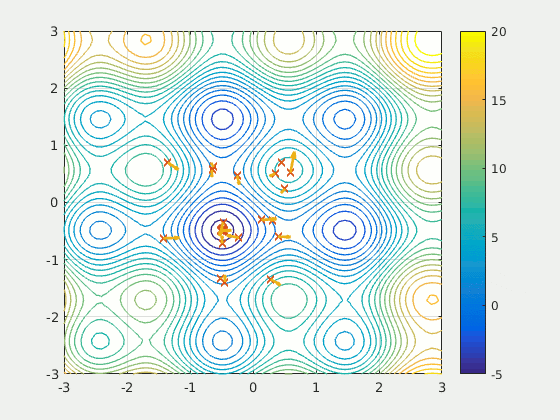
\includegraphics[width=0.45\textwidth]{./Figures/ejemplopso/capas-79.png}
}
    % \begin{subfigure}[t]{0.45\textwidth}
        %\caption{Enhanced Image using \cite{morepso}. $\mathscr{H_Y}=0.788927$. $SSIM_R=0.000204143$. $SSIM_G=0.0000526475$. $SSIM_B=0.0000518143$}
        \label{fig:calhouse233orig}
        \end{subfigure}
\begin{subfigure}[]{
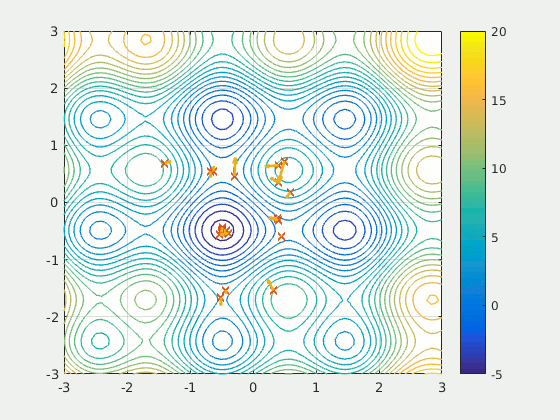
\includegraphics[width=0.45\textwidth]{./Figures/ejemplopso/capas-95.png}
}
    % \begin{subfigure}[t]{0.45\textwidth}
        %\caption{Enhanced Image using \cite{morepso}. $\mathscr{H_Y}=0.788927$. $SSIM_R=0.000204143$. $SSIM_G=0.0000526475$. $SSIM_B=0.0000518143$}
        \label{fig:calhouse23129}
        \end{subfigure}
    ~ %add desired spacing between images. e. g. ~. \quad. \qquad. \hfill etc. 
    %(or a blank line to force the subfigure onto a new line)
    \begin{subfigure}[]{
    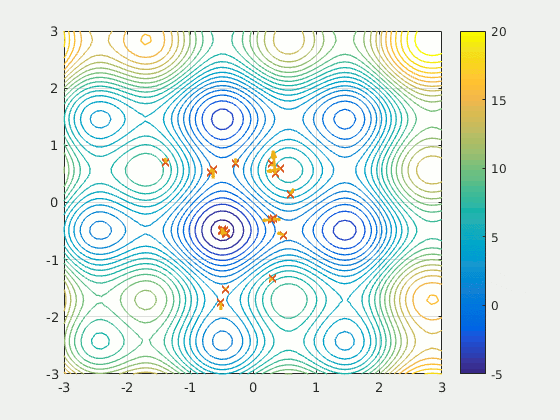
\includegraphics[width=0.45\textwidth]{./Figures/ejemplopso/capas-99.png}
    }
    % \begin{subfigure}[t]{0.45\textwidth}
%        \caption{Enhanced Image.  $\mathscr{H_Y}=0.0350595$. $SSIM_R=0.416776$. $SSIM_G=0.403636$. $SSIM_B=0.417654$}
\label{fig:calhouse231102}
\end{subfigure}
        \caption{Comportamiento de partículas en $PSO$ monobjetivo a través de la serie de iteraciones.}
        \label{fig:comportamientopso}
\end{figure}



%Here, $\vv{v}$ is a factor known as the velocity, and is given by:

% \begin{equation}\label{eq:velocidad1}
%  \vv{v}_i(t) = w \cdot (t-1) + C_1 \cdot r_1 \cdot (\vv{x}_{p_i} - \vv{x}_i) + C_2 \cdot r_2 \cdot (\vv{x}_{g_i} - \vv{x_i}) \text{,}
% \end{equation}
% where $\vv{x}_{p_i}$ is the best solution that $\vv{x}_i$ has found so far, $\vv{x}_{g_i}$ is the best solution that the entire swarm has found at the current iteration, $w$ is a coeficient known as the \textit{inertia weight}, which controls the search speed rate of $PSO$; $r_1$ and $r_2$ are random numbers between $[0,1]$. Finally, $C_1$ and $C_2$ are coefficient which control the weight between global and local particles during the search.

% In $MOPSO$, a \textit{constriction coefficient} $\chi$ is adopted in order to control the particle's velocity, as described below:

% \begin{equation}
% \chi = \frac{2}{2 - \varphi - \sqrt{\varphi^2 - 4 \varphi}}
% \end{equation}

donde

% where

\begin{equation}
% \[
\varphi= 
\begin{cases}
C_1 + C_2 & \text{if } C_1 + C_2 > 4\\
0,              & \text{if } C_1 + C_2 \leq 4
\end{cases}
% \]
\end{equation}

Además, la velocidad en $MOPSO$ se acota con la siguiente ecuación de constricción de velocidad:

% Furthermore, the velocity in $MOPSO$ is bounded by the following \textit{velocity constriction} equation:
\begin{equation}\label{eq:restricciondelta}
% \[
v_{i,j}(t)= 
\begin{cases}
delta_j & \text{if } v_{i,j}(t) > delta_j\\
-delta_j,      & \text{if } v_{i,j}(t) \leq delta_j \\
v_{i,j}(t),      & \text{otherwise }
\end{cases}
% \]
\end{equation}

donde

% where

\begin{equation}
delta_j=\frac{upper\_limit_j - lower\_limit_j}{2}
\end{equation}

\section{Métricas de Optimización}

\subsection{Entropía de la imagen}
%\subsection{Entropy of image}

La entropía de la imagen \cite{108593} es una métrica que mide cuánta información está representada dentro de la imagen. La entropía y el contraste se relacionan de manera muy cercana a la distribución de intensidad de las imágenes, por lo que esta métrica es capaz de verificar las variaciones de contraste como consecuencia de las transformaciones de la imagen.

%Entropy of image \cite{108593} is a metric that measures how much information is represented within an image. Entropy and contrast are closely related to the intensity distribution of images, so this metric is able to assess contrast variations as a consecuence of image transformations.

Primero, es necesario definir el \textit{Histograma} de intensidades de una imagen $H$ como sigue: Sea $c_1, c_2, ..., c_n$ el conteo de pixeles con intensidades $i_1, i_2, ..., i_n$ respectivamente, y sea también:

%First, we need to define the \textit{Histogram} of intensities of an image $H$ as follows: Let $c_1, c_2, ..., c_n$ the count of pixels with intensity $i_1, i_2, ..., i_n$ respectively, and also let

\begin{equation}
p_i=\frac{c_i}{N}, \qquad \sum_{i=1}^n c_i = N, \qquad i= 1,2, ..., n,
\end{equation}

donde $N$ es la suma total de pixeles mostrados en una imagen $I$ y $n$ es cada nivel de intensidad representable por el espacio de colores de $I$. Entonces, $H$ se define como la distribución de probabilidad en el que cada $p_i$ representa la probabilidad de ocurrencia de una intensidad $i$. Entonces, la Entropía de la Imagen se define de la siguiente manera:

%where $N$ is the total sum of pixels shown in an image $I$ and $n$ is every intensity level representable by the color space of $I$. Then $H$ is defined as a probability distribution in which every $p_i$ represents the probability of occurrence of an intensity $i$. Then, Entropy of Image is defined as below:

\begin{equation}
\mathscr{H}\label{symbol:entropia}= -\sum_{i=0}^{n-1} p_i \text{log}_2(p_i) \qquad \mathscr{H} \in \{0,...,\text{log}_2(n)\}
\end{equation}

\begin{figure}[H]
\centering
    %\begin{subfigure}[t]{0.45\textwidth}
    % \begin{subfigure}[]{
    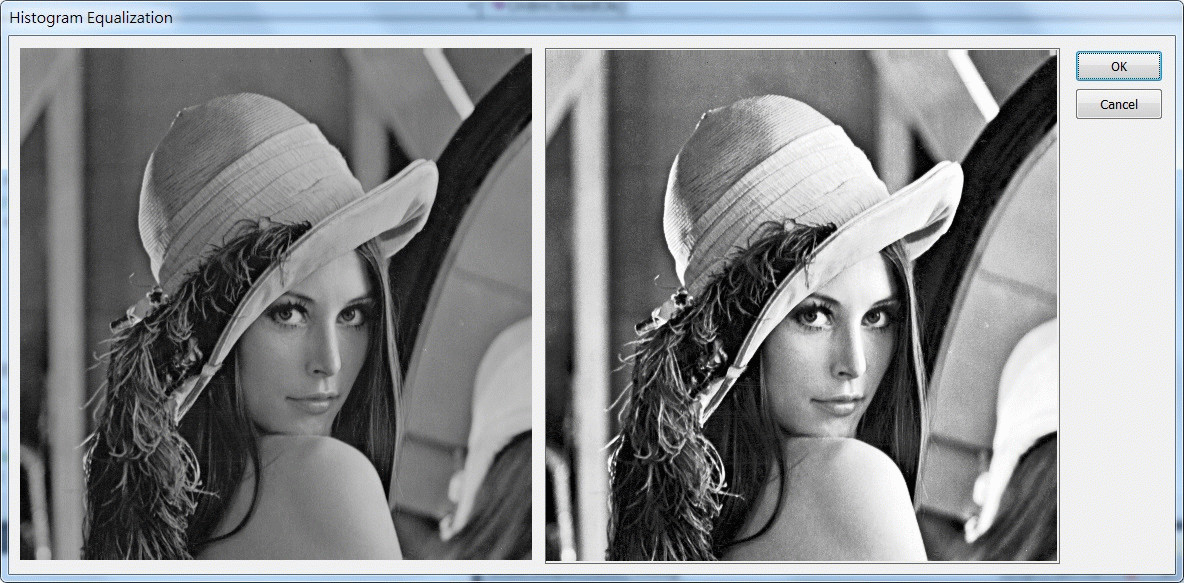
\includegraphics[width=0.85\textwidth]{./Figures/lennaejemplo.jpg}
    % }
        \caption{Datos de $\mathscr{H}$ para una imagen de ejemplo. A la derecha $\mathscr{H}$, a la izquierda $\mathscr{H}=$}
        \label{fig:lenaejemploentropia}
\end{figure}

\subsection{Índice de Similaridad Estructural}

El \textit{Índice de Similaridad Estructural} ($SSIM$) \cite{wang2004image} es una métrica bien conocida que mide atributos importantes de la imagen tales como la \textit{Luminancia, Contraste}y la \textit{Estructura}. $SSIM$ tiene como objetivo principal medir la distorsión agregada a la imagen como consecuencia del proceso de Mejora del Contraste. $SSIM$ es calculado por regiones, por lo tanto, dadas dos imágenes $I_x$ y $T_y$ que representan una imagen original y una mejorada, respectivamente, el índice $SSIM$ se define como se muestra abajo: 

%The \textit{Structural Similarity Index} ($SSIM$) \cite{wang2004image} is a well known metric that measures important image's attributes such as \textit{Luminance, Contrast} and \textit{Structure}. SSIM main aim is to measure the distortion added to the image as a consecuence of the CE proccess. $SSIM$ is calculated by windows, so given two images $I_x$ and $T_y$ which represent an original and an enhanced image, respectively, the $SSIM$ index is defined as below:

\begin{equation}
SSIM(I,T)\label{symbol:ssim} = \frac{(2\mu_{I_x} \mu_{T_y}+E_1)(2\sigma_{I_xT_y}+E_2)}{(\mu^2_{I_x}+\mu^2_{T_y}+E_1)(\sigma^2_{I_x} + \sigma^2_{T_y}+E_2)} \qquad SSIM \in [0,1]
\end{equation}

donde $\mu_{I_x}$\label{symbol:ssimmui}, $\mu_{T_y}$\label{symbol:ssimmut} son los promedios de intensidad de $I_x$ y $T_y$, respectivamente; $\sigma^2_{I_x}$\label{symbol:ssimsigmat} y $\sigma^2_{T_y}$\label{symbol:ssimsigmat} son las varianzas de intensidad para $I_x$ y $T_y$, respectivamente; $\sigma_{I_xT_y}$\label{symbol:ssimsigmait} es la covarianza entre las intensidades $I_x$ y $T_y$. $E_1=(K_1L^2)$, donde $L$ es el rango dinámico de intensidades de los pixeles de la imagen, y $K_1 \ll 1$ es una constante pequeña; $E_2=(K_2L)^2$, y $K_2 \ll 1$; tanto $E_1$ como $E_2$ son constantes utilizadas para estabilizar la división cuando el denominador se acerca a cero.

\begin{figure}[H]
\centering
    %\begin{subfigure}[t]{0.45\textwidth}
    % \begin{subfigure}[]{
    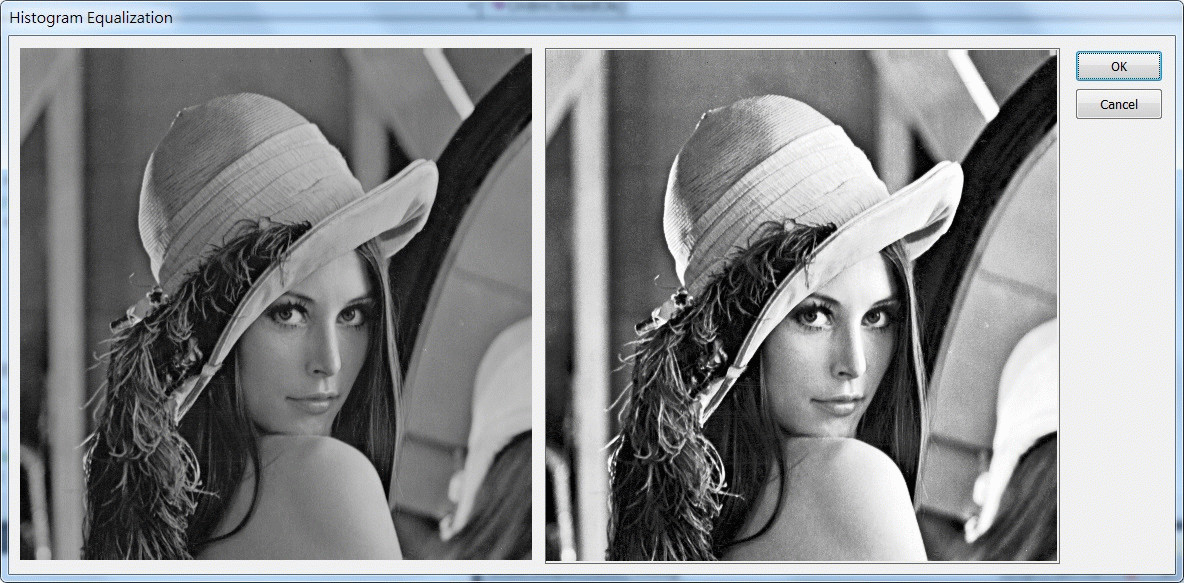
\includegraphics[width=0.85\textwidth]{./Figures/lennaejemplo.jpg}
    % }
        \caption{Datos de $SSIM$ para una imagen de ejemplo. A la derecha $SSIM$, a la izquierda $SSIM$}
        \label{fig:lenaejemploSSIM}
\end{figure}


%where $\mu_{I_x}$, $\mu_{T_y}$ is the intensity averages of $I_x$ and $T_y$, respectively; $\sigma^2_{I_x}$ and  $\sigma^2_{T_y}$ are the intensity variances for $I_x$ and $T_y$, respectively; $\sigma_{I_xT_y}$ is the covariance between $I_x$ and $T_y$ intensities. $E_1=(K_1L^2)$, where $L$ is the dynamic range of intensities of image's pixels, and $K_1 \ll 1$ is a small constant; $E_2=(K_2L)^2$, and $K_2 \ll 1$; both $E_1$ and $E_2$ are constants used to stabilize division when denominator is close to zero.


%En la vida cotiana las imágenes en color están involucradas en todos los aspectos. La televisión, la fotografía y la impresión son actividades diarias en la vida de un ser humano. La percepción del color es un fenómeno fascinante y complicado que ha ocupado el interés de los científicos, psicólogos, filósofos y artistas durante cientos de años \citep{burger2016digital}.

% En este capítulo se presentan los principales conceptos teóricos de la morfología matemática y su extensión para imágenes en color.

% \section{Imagen digital}

% Una imagen digital $f$\label{symbol:ioriginal} está definida por una función bidimensional cuyo valor es \textit{n}-dimensional $f:\mathbb{Z}^{2}\longmapsto \mathbb{R}^{n}$\label{symbol:intset}, donde cada píxel $(u,v)\in \mathbb{Z}^{2}$ tiene un valor asociado $m=(c_{1},c_{2},\cdots,c_{n})$\label{symbol:valorm}. Si $n=1$ la imagen es binaria o en escala de grises, por tanto los rango de valores del componente $c$\label{symbol:valorc} van entre 0 y 1, o entre 0 y 255. Si $n>1$ la imagen es en color y los rangos de valores de cada componente $c_{k}$ dependen del espacio de color elegido para su representación. Los espacios de color son varios, como el RGB, HSI, HSV, entre otros \cite{ortiz2002procesamiento,gonzalez2007image}. En la Figura \ref{f:I50} se visualiza una imagen en color de \textit{Lenna}.

% \begin{figure}[!ht]
% 	\centering
% 	\includegraphics[width=0.3\textwidth]{./Figures/lenna.jpg}
% 	\caption{Imagen en color de \textit{Lenna}.}
% 	\label{f:I50}
% \end{figure}

% \section{Histograma}

% Los histogramas son distribuciones de frecuencia, describen la frecuencia de los valores de intensidad que se producen en una imagen. Sea la imagen $f = (f_{1},f_{2},\cdots,f_{n})$. El histograma, del $k-$ésimo componente de la imagen $f_{k}$\label{symbol:fk} con $k={1,2,\cdots,n}$, es una función discreta que se define como:

% \begin{equation}
% 	\label{symbol:hfk}
% 	h_{f_{k}}(j)=n_{j},
% \end{equation}

% donde $j$\label{symbol:j} representa $j-$ésimo nivel de intensidad en un rango de [0,L-1] de $f_{k}$, $n_{j}$\label{symbol:nj} es la cantidad de ocurrencia de la intensidad $j$ en $f_{k}$. $L$\label{symbol:L} es el máximo nivel de intensidad, teniendo en cuenta una configuración de 8 bits por cada componente de $f$ tendremos que $L=2^{8}=256$.

% En las Figuras \ref{f:I51}, \ref{f:I52} y \ref{f:I53} se muestran las imágenes de \textit{Lenna} por cada componente R, G y B con sus respectivos histogramas.
% %Histogramas

% \begin{figure}[!ht]
% 	\centering
% 	\subfigure[]{\includegraphics[width = 2.5in]{./Figures/lenna_R.jpg}}
% 	\subfigure[]{\includegraphics[width = 2.5in]{./Figures/lenna_R_H.jpg}}
% 	\caption{Imágenes de \text{lenna} del componente R con su respectivo histograma.}
% 	\label{f:I51}
% \end{figure}

% \begin{figure}[!ht]
% 	\centering
% 	\subfigure[]{\includegraphics[width = 2.5in]{./Figures/lenna_G.jpg}}
% 	\subfigure[]{\includegraphics[width = 2.5in]{./Figures/lenna_G_H.jpg}}
% 	\caption{Imágenes de \text{lenna} del componente G con su respectivo histograma.}
% 	\label{f:I52}
% \end{figure}

% \begin{figure}[!ht]
% 	\centering
% 	\subfigure[]{\includegraphics[width = 2.5in]{./Figures/lenna_B.jpg}}
% 	\subfigure[]{\includegraphics[width = 2.5in]{./Figures/lenna_B_H.jpg}}
% 	\caption{Imágenes de \text{lenna} del componente B con su respectivo histograma.}
% 	\label{f:I53}
% \end{figure}


% Los histogramas se utilizan a menudo para determinar si una imagen está haciendo un uso efectivo de su rango de intensidad examinando el tamaño y la uniformidad de la distribución del histograma, así también nos permite detectar problemas que se originan durante la adquisición de la imagen, como los que implican el contraste y rango dinámico.

% \section{Contraste de una imagen}
% %\textcolor{Micolor1}{El contraste se define como la diferencia en luminancia media entre un objeto y su entorno \cite{wang2003chromosome}} 
% El contraste se entiende como una combinación del intervalo de valores de intensidad efectivamente utilizados dentro de una imagen dada y la diferencia entre los valores de píxel máximo y mínimo de la imagen \cite{burger2016digital}, esta diferencia nos permite distinguir los objetos del fondo de una imagen. Cuando una imagen posee un alto contraste, las zonas claras se diferencian mejor de las zonas oscuras. En la Figura \ref{f:I54} podemos ver una imagen con un bajo contraste donde el auto se visualiza deficientemente porque los niveles de grises son muy semejantes, por tal motivo el histograma se encuentra concentrado en una sección.

% \begin{figure}[!ht]
% 	\centering
% 	\subfigure[]{\includegraphics[width = 2.5in]{./Figures/29030bc.jpg}}
% 	\subfigure[]{\includegraphics[width = 2.5in]{./Figures/29030bc_H.jpg}}
% 	\caption{Imagen con bajo contraste con su respectivo histograma. Donde (a) es la imagen con bajo contraste y (b) es el histograma de la imagen con bajo contraste.}
% 	\label{f:I54}
% \end{figure}

% En la Figura \ref{f:I55} podemos ver una imagen con un alto contraste donde el auto se visualiza mucho mejor y el histograma nos muestra que las intensidades de gris se distribuyen en todo el rango.

% \begin{figure}[!ht]
% 	\centering
% 	\subfigure[]{\includegraphics[width = 2.5in]{./Figures/29030ac.jpg}}
% 	\subfigure[]{\includegraphics[width = 2.5in]{./Figures/29030ac_H.jpg}}
% 	\caption{Imagen con alto contraste con su respectivo histograma. Donde (a) es la imagen con alto contraste y (b) es el histograma de la imagen con alto contraste.}
% 	\label{f:I55}
% \end{figure}

% \section{Espacios de color} 

% Los espacios de color son arreglos tridimensionales de sensaciones de color. Los colores se especifican por puntos en estos espacios.
% En este trabajo se utilizan el espacio de color RGB, por estar orientado al hardware, y los espacios de color HSI y HSV, por estar orientados al usuario. 


% \subsection{Espacio de color RGB} 

% En el espacio de color RGB los colores se codifican como combinaciones de los tres colores primarios: rojo (R), verde (G) y azul (B). Este esquema es ampliamente utilizado para la transmisión, representación y almacenamiento de imágenes en color tanto en dispositivos analógicos como televisores y dispositivos digitales como ordenadores, cámaras digitales y escáneres. Por tal motivo, muchos programas de procesamiento de imágenes y gráficos utilizan el esquema RGB como su representación interna para las imágenes en color.

% RGB es un sistema de color aditivo, lo que significa que todos los colores comienzan con negro y se crean mediante la adición de los colores primarios. Para crear diferentes colores, se modifican la intensidad de cada uno de estos colores independientemente. La intensidad distinta de cada color primario controla la sombra y el brillo del color resultante. Los colores gris y blanco se crean mezclando los tres colores primarios con la misma intensidad.

% El espacio de color RGB se puede visualizar como un cubo de unidad tridimensional en el que los tres colores primarios forman el eje de coordenadas \cite{burger2016digital}.

% En la Figura \ref{f:I40} se muestra el espacio de color RGB.

% \begin{figure}[!ht]
% 	\centering
% 	\includegraphics[width=0.6\textwidth]{./Figures/RGB.JPG}
% 	\caption{Espacio de color RGB.}
% 	\label{f:I40}
% \end{figure}

% \subsection{Familia de espacios de color HSI}

% El ojo del ser humano no reconoce un color por tener una cantidad de componente roja, verde o azul. El ojo del ser humano emplea atributos perceptuales de luminancia o intensidad (I, V o L), saturación (S) y matiz (M). Los modelos espacios de color HSI, HSV y sus variantes, codifican el color con los atributos de luminancia o intensidad, saturación y matiz, y se definen como espacios intuitivos u orientados a usuario, pues son los óptimos para interacción humana. El matiz H representa la impresión relacionada con la longitud de onda dominante del estímulo de color. La saturación corresponde a la pureza relativa del color y en el caso de un color puro es igual al 100\%. Los colores con saturación cero son los niveles de gris. La luminancia o intensidad máxima se detecta como blanco puro, la luminancia o intensidad mínima como negro puro \cite{sangwine2012colour}.

% Una transformación de coordenadas hace posible que la familia de espacios HSI se derive del espacio de color RGB. Mediante la transformación el cubo RGB pasa a tener forma cilíndrica. Los espacios de la familia HSI están compuestos por los espacios HSI, HSV y HLS; estos espacios poseen aspecto cilíndrico, de forma que la saturación se corresponde con un valor de distancia radial, mientras que el matiz es función de ángulo en el sistema de coordenadas polar. La intensidad es la distancia a lo largo del eje perpendicular al plano de coordenadas polares. Para un estudio más profundo de estos espacios de color el lector puede ver \cite{ortiz2002procesamiento,gonzalez2007image}.

% En la Figura \ref{f:I41} se muestran (a) el esspacio de color HSI y (b) el espacio de color HSV.

% \begin{figure}[!ht]
% 	\centering
% 	\subfigure[]{\includegraphics[width = 2.5in]{./Figures/HSI.JPG}}
% 	\subfigure[]{\includegraphics[width = 2.5in]{./Figures/HSV.JPG}}
% 	\caption{(a) Espacio de color HSI y (b) espacio de color HSV.}
% 	\label{f:I41}
% \end{figure}

% La utilización de un espacio de color dentro de una aplicación, en el procesamiento de imágenes, depende de la elección que se realice. Ésta elección depende a su vez de las propiedades del modelo como de las características de la aplicación. En las siguientes secciones trataremos sobre la morfología matemática para imágenes en escala de grises y su extensión para imágenes en color mediante la selección de un orden dentro de un espacio de color.

% \section{Morfología matemática}

% La morfología matemática es una potente herramienta para diversas aplicaciones de procesamiento de imágenes y visión por computador. La morfología se ha utilizado para realizar mejora del contraste, supresión de ruido, análisis de texturas, análisis de formas, detección de bordes, esqueletización y filtrado multiescalar para aplicaciones tales como imágenes médicas, procesamiento de imágenes geológicas, inspección industrial automatizada, compresión de imágenes, análisis de señales, entre otros \cite{serra1982image,ortiz2002procesamiento,sangwine2012colour}.

% La morfología en escala de grises es una generalización de la morfología binaria y los procedimientos diseñados son válidos para ésta \cite{burger2016digital}. La morfología matemática se sustenta sobre dos transformaciones morfológicas básicas que son la erosión (minimización) y la dilatación (maximización). Las transformaciones morfológicas tienen como objetivo extraer estructuras geométricas en los conjuntos sobre los que se opera (imagen), ésto lo realiza utilizando otro conjunto conocido denominado elemento estructurante. El tamaño y la forma del elemento estructurante se elige de acuerdo a la forma que se quiere obtener del conjunto y sobre el cual se va a interaccionar.

% \subsection{Elemento estructurante}
% La imagen se transforma por otro conjunto, conocido como elemento estructurante. La forma y el tamaño del elemento estructurante determinan la imagen resultante. El elemento estructurante $g$\label{symbol:se} se define como \cite{burger2016digital}:
% \[  
% g(s,t) \in \mathbb{R},\textit{ para } (s,t) \in \mathbb{Z}^{2}, 
% \]
% y sus valores pueden ser positivos, negativos o cero. En la Figura \ref{f:I60} se muestra un ejemplo de formas básicas de elementos estructurantes planos y en la Figura \ref{f:I86} se muestra la representación matricial de un elemento estructurante cuadrado y plano de $3 \times 3$.

% \begin{figure}[!ht]
% 	\centering
% 	\includegraphics[width=0.4\textwidth]{./Figures/se_1.png}
% 	\caption{Ejemplo de formas básicas de elementos estructurantes planos.}
% 	\label{f:I60}
% \end{figure}

% \begin{figure}[!ht]
% 	\centering
% 	\includegraphics[width=0.2\textwidth]{./Figures/se.JPG}
% 	\caption{Elemento estructurante cuadrado y plano de $3 \times 3$. El origen se sitúa en el centro.}
% 	\label{f:I86}
% \end{figure}

% \subsection{Dilatación y Erosión}

% Sea la imagen $f$ cuyo píxel está representado por las coordenadas espaciales $(u,v)$\label{symbol:uv} y un elemento estructurante $g$ cuya coordenada espacial está representado por $(s,t)$\label{symbol:st}. La dilatación ($f \oplus g$)\label{symbol:dil} y la erosión ($f \ominus g$)\label{symbol:ero} de la imagen $f$ por $g$  se define como \cite{burger2016digital}:

% \begin{equation} \label{dil}
% 	\begin{split}
% 		(f \oplus g)(u,v) =\max_{(s,t) \in g}\{f(u+s,v+t) + g(s,t)\},
% 	\end{split}
% \end{equation}

% \begin{equation} \label{ero}
% 	\begin{split}
% 		(f \ominus g)(u,v)=\min_{(s,t)\in g}\{f(u+s,v+t) - g(s,t)\}.
% 	\end{split}
% \end{equation}

% En la Figura \ref{f:I81} visualizamos las operaciones morfológicas de erosión y dilatación de la imagen \textit{388067} por un elemento estructurante cuadrado $g$ de $3 \times 3$. Los detalles claros y oscuros de la imagen se reducen con las operaciones de erosión y dilatación.

% \begin{figure}[!ht]
% 	\centering
% 	\subfigure[]{\includegraphics[width = 1.72in]{./Figures/388067.jpg}}
% 	\subfigure[]{\includegraphics[width = 1.72in]{./Figures/388067_ero.jpg}}
% 	\subfigure[]{\includegraphics[width = 1.72in]{./Figures/388067_dil.jpg}}
% 	\caption{Operaciones morfológicas de erosión y dilatación. Donde (a) es la imagen \textit{388067}, (b) es la imagen erosionada y (c) la imagen dilatada con un elemento estructurante cuadrado $g$ de $3\times 3$.}
% 	\label{f:I81}
% \end{figure}

% Con los operadores de dilatación y erosión puede extenderse toda la matemática morfológica.

% \subsection{Apertura y cierre}

% La apertura ($f \circ g$)\label{symbol:ape} y el cierre ($f \bullet g$)\label{symbol:cie} de $f$ por $g$ se definen a partir de los conceptos de dilatación y erosión como sigue \cite{gonzalez2007image}:
% \begin{equation}
% 	\label{ape}
% 	f \circ g = (f \ominus g) \oplus g,
% \end{equation}
% \begin{equation}
% 	\label{cie}
% 	f \bullet g = (f \oplus g) \ominus g.
% \end{equation}

% En la Figura \ref{f:I82} visualizamos las operaciones morfológicas de apertura y cierre de la imagen \textit{388067} por un elemento estructurante cuadrado $g$ de $3 \times 3$. La apertura morfológica se utiliza para borrar detalles claros y el cierre morfológico se utiliza para borrar detalles oscuros, que sean pequeños en comparación con el elemento estructurante.

% \begin{figure}[!ht]
% 	\centering
% 	\subfigure[]{\includegraphics[width = 1.72in]{./Figures/388067.jpg}}
% 	\subfigure[]{\includegraphics[width = 1.72in]{./Figures/388067_ape.jpg}}
% 	\subfigure[]{\includegraphics[width = 1.72in]{./Figures/388067_cie.jpg}}
% 	\caption{Operaciones morfológicas de apertura y cierre. Donde (a) es la imagen \textit{388067}, (b) es apertura morfológica y (c) es el cierre morfológico de la imagen \textit{388067} con un elemento estructurante cuadrado $g$ de $3\times 3$.}
% 	\label{f:I82}
% \end{figure}

% \subsection{Transformada de top-hat}

% A partir de la apertura y el cierre se define la transformada de top-hat por apertura $WTH$\label{symbol:wth} y la transformada de top-hat por cierre $BTH$\label{symbol:bth} de la imagen $f$ como sigue \cite{gonzalez2007image}:

% \begin{equation}
% 	\label{wth}
% 	WTH = f - f \circ g,
% \end{equation}

% \begin{equation}
% 	\label{bth}
% 	BTH = f \bullet g - f.
% \end{equation}

% En la Figura \ref{f:I83} visualizamos las operaciones de la transformada de top-hat por apertura y cierre de la imagen \textit{388067} con un elemento estructurante cuadrado $g$ de $3 \times 3$.

% \begin{figure}[!ht]
% 	\centering
% 	\subfigure[]{\includegraphics[width = 1.72in]{./Figures/388067_wth.jpg}}
% 	\subfigure[]{\includegraphics[width = 1.72in]{./Figures/388067_bth.jpg}}
% 	\caption{Transformada de top-hat por apertura y cierre.}
% 	\label{f:I83}
% \end{figure}

% En la apertura y el cierre las regiones brillantes y oscuras de la imagen se atenúan. Luego, con $WTH$ se obtienen las regiones brillantes y con $BTH$ se obtienen las regiones oscuras de la imagen.

% \subsection{Mejora de contraste de una imagen basado en la transformada de top-hat}

% La mejora del contraste de la imagen $f$ basado en la transformada de top-hat consiste en añadir regiones brillantes y sustraer regiones oscuras a la imagen $f$ como sigue \cite{soille2013morphological}:

% \begin{equation}
% 	\label{fen}
% 	f_{E} = f + WTH - BTH,
% \end{equation}
% donde $f_{E}$\label{symbol:fen} es la imagen resultante con mejora de contraste.

% En la Figura \ref{f:I87} se muestra el esquema de mejora de contraste basado en la transformada de top-hat.

% \begin{figure}[!ht]
% 	\centering
% 	\includegraphics[width=0.5\textwidth]{./Figures/mejora_contraste.JPG}
% 	\caption{Esquema de mejora de contraste basado en la transformada de top-hat.}
% 	\label{f:I87}
% \end{figure}

% \section{Morfología matemática en color}

% La morfología matemática en color es una extensión de la morfología en escala de grises. Serra et. al. \cite{serra1988image} discute la generalización de la morfología a sus elementos más básicos mediante una relación de orden, un supremo y un ínfimo que pertenece a un orden y la posibilidad de admitir una infinidad de operaciones.

% En las imágenes en color, el color se representa de manera vectorial y no existe un orden natural para ordenar dos o más colores, por tal motivo la extensión de la matemática morfológica en color no es trivial. Para obtener el máximo y mínimo por medio de las operaciones de dilatación y erosión es necesario ordenar los componentes de los vectores de la imagen en color.

% \subsection{Tratamiento de las imágenes en color}

% Las imágenes en color pueden ser tratadas en forma marginal o vectorial. Si las operaciones de escala de grises se aplican individualmente a cada canal del color en RGB, el tratamiento es marginal. Para el tratamiento vectorial de las imágenes en color se requiere del establecimiento de un orden entre todos los píxeles de las imágenes sobre el cual se realizan las operaciones \cite{ortiz2002procesamiento} sea el espacio de color que se elija.

% En la Figura \ref{f:I70} se muestran los esquemas de tratamiento de las imágenes en color.

% \begin{figure}[!ht]
% 	\centering
% 	\subfigure[]{\includegraphics[width = 2.5in]{./Figures/marginal.JPG}}
% 	\subfigure[]{\includegraphics[width = 2.5in]{./Figures/vectorial.JPG}}
% 	\caption{(a) Esquema de tratamiento marginal y (b) esquema de tratamiento vectorial.}
% 	\label{f:I70}
% \end{figure}

% \subsection{Métodos de ordenamiento}
% %\textcolor{Micolor1}{ 
% %El orden de los componentes de los vectores se puede realizar de varias maneras. Los métodos de ordenamiento vectorial se caracterizan por ser definidas como de preorden, orden, total o parcial \cite{ortiz2002procesamiento}. Cabe destacar que cada ordenamiento arrojará resultados diferentes.
% %Para aplicar la morfología matemática a imágenes en color necesitamos adoptar un orden dentro de un espacio de color. A continuación describiremos los órdenes utilizados en este trabajo para los experimentos.
% %%Para aplicar la morfología matemática a un espacio de color necesitamos adoptar un orden dentro de ésta. A continuación describiremos los órdenes utilizados en este trabajo para los experimentos.
% %}

% El ordenamiento de los componentes de los vectores se puede realizar de varias maneras, por un componente, distancia euclidiana, orden canónico, orden lexicográfico, entre otros \cite{ortiz2002procesamiento}. En este trabajo se utilizaron estrategias de orden total, para garantizar la unicidad del ínfimo y el supremo, dentro de los espacios de color RGB, HSI y HSV. Cabe destacar que cada ordenamiento arrojará resultados diferentes. A continuación describiremos los métodos de ordenamientos utilizados para los experimentos de este trabajo.

% \subsubsection{Método de ordenamiento propuesto por Tobar et. al. \cite{tobar2006estudio} (TPSA)}
% \label{symbol:tpsa}

% Este método propone no dar mayor peso a ninguno de los componentes del espacio de color RGB, utilizando un orden total \cite{tobar2006estudio}. Donde dados dos píxeles $p$\label{symbol:puv} y $q$\label{symbol:quv} con sus valores asociados $m_{1}=(r_{1},g_{1},b_{1})$ y $m_{2}=(r_{2},g_{2},b_{2})$, donde $a_{1} = r_{1}+g_{1}+b_{1}$, $d_{1} = r_{2}+g_{2}+b_{2}$, $a_{2} = g_{1}+b_{1}$, $d_{2} = g_{2}+b_{2}$, $a_{3} = b_{1}$ y $d_{3} = b_{2}$, la ecuación se define como:

% \begin{equation}
% 	p \leq q\equiv
% 	\label{e1}
% 	\left\{\begin{matrix}
% 		a_{1}<d_{1}\text{ (1) }\\
% 		o\\  
% 		a_{1}=d_{1} \wedge a_{2}<d_{2}\text{ (2) } \\ 
% 		o\\ 
% 		a_{1}=d_{1} \wedge a_{2}=d_{2} \wedge a_{3} \leq d_{3}\text{ (3) } 
% 	\end{matrix}\right.
% \end{equation}

% En la Figura \ref{f:I91} se muestran (a) la imagen original \textit{16068} en color, (b) la imagen dilatada y (c) la imagen erosionada con un elemento estructurante $g$ cuadrado de $3 \times 3$, teniendo en cuenta el método de ordenamiento TPSA.

% \begin{figure}[!ht]
% 	\centering
% 	\subfigure[]{\includegraphics[width=0.3\textwidth]{./Figures/16068.jpg}}
% 	\subfigure[]{\includegraphics[width=0.3\textwidth]{./Figures/16068_dil_RGB.jpg}}
% 	\subfigure[]{\includegraphics[width=0.3\textwidth]{./Figures/16068_ero_RGB.jpg}}
% 	\caption{Dilatación y erosión de la imagen con un elemento estructurante cuadrado de $3 \times 3$, teniendo en cuenta el método de ordenamiento TPSA.}
% 	\label{f:I91}
% \end{figure}

% \subsubsection{Método de ordenamiento propuesto por Vazquez et. al \cite{noguera2014color} (JLVN)}
% \label{symbol:jlvn}

% Este método propuesto por Vazquez et. al. \cite{noguera2014color}, permite evitar dar mayor importancia a uno de los componentes de la imagen. Introduce un nuevo valor en el primer lugar de la cascada lexicográfica. Sea la imagen $f$ con sus respectivos canales,
% \[
% \label{symbol:fk2}
% f_{k}=(f_{1},f_{2},f_{3})\text{ }\forall_{k}=1:k\text{ } \wedge \text{ } k=3,
% \]
% donde la función de pesos $w$\label{symbol:wp} que adoptaremos para el experimento se define como:
% \begin{equation}
% 	w_{k}(f_{k})=\sum_{u=0}^{M-1}\sum_{v=0}^{N-1}(u,v)_{k}\text{ }\forall_{k}=1:k.
% \end{equation}

% La transformada $T(f)$\label{symbol:tf} es el nuevo valor que se introduce en el primer lugar de la cascada lexicográfica se define como:
% \begin{equation}
% 	T(f)(u,v)=\sum_{k=1}^{3}w_{k} \times f_{k}(u,v),
% \end{equation}
% por tanto el orden lexicográfico queda definido como:
% \begin{equation}
% 	p \leq q \Leftrightarrow [T(f),p_{1},p_{2},p_{3}]  \leq  [T(f_{E}),q_{1},q_{2},q_{3}],
% \end{equation}
% donde el píxel $p\in f$ y $q\in f_{E}$.

% El ordenamiento lexicográfico que utilizaremos para las pruebas en el espacio de color RGB será $T\longrightarrow R\longrightarrow G \longrightarrow B$.

% En la Figura \ref{f:I92} se muestran (a) la imagen original \textit{16068} en color, (b) la imagen dilatada y (c) la imagen erosionada con un elemento estructurante $g$ cuadrado de $3 \times 3$, teniendo en cuenta el método de ordenamiento JLVN.

% \begin{figure}[H]
% 	\centering
% 	\subfigure[]{\includegraphics[width=0.25\textwidth]{./Figures/388067_C.jpg}}
% 	\subfigure[]{\includegraphics[width=0.25\textwidth]{./Figures/388067_dil_TRGB.jpg}}
% 	\subfigure[]{\includegraphics[width=0.25\textwidth]{./Figures/388067_ero_TRGB.jpg}}
% 	\caption{Dilatación y erosión de la imagen con un elemento estructurante cuadrado de $3 \times 3$, teniendo en cuenta el método de ordenamiento JLVN.}
% 	\label{f:I92}
% \end{figure}

% \subsubsection{Método de ordenamiento lexicográfico}
% \label{symbol:ihs}
% En los espacios de color HSI y HSV utilizaremos el método de ordenamiento lexicográfico, que consiste en la asignación de prioridades de los componentes del vector, para que unos posean más importancias que otros. Los ordenamientos seleccionados son el IHS ($I\longrightarrow H\longrightarrow S$) y el VHS ($V\longrightarrow H\longrightarrow S$). Estos ordenamientos serán adecuado para preservar los contornos de los objetos de la imagen \cite{ortiz2002procesamiento}.

% En la Figura \ref{f:I93} se muestran (a) la imagen original \textit{16068} en color, (b) la imagen dilatada y (c) la imagen erosionada con un elemento estructurante $g$ cuadrado de $3 \times 3$, teniendo en cuenta el método de ordenamiento IHS.

% \begin{figure}[H]
% 	\centering
% 	\subfigure[]{\includegraphics[width=0.25\textwidth]{./Figures/388006.jpg}}
% 	\subfigure[]{\includegraphics[width=0.25\textwidth]{./Figures/388006_dil_IHS.jpg}}
% 	\subfigure[]{\includegraphics[width=0.25\textwidth]{./Figures/388006_ero_IHS.jpg}}
% 	\caption{Dilatación y erosión de la imagen con un elemento estructurante cuadrado de $3 \times 3$, teniendo en cuenta el método de ordenamiento IHS.}
% 	\label{f:I93}
% \end{figure}

% \section{Resumen}
% Este capítulo presentó una introducción a las imágenes en color y a los conceptos de las operaciones de la morfología matemática. La extensión de la morfología matemática en color se realizó mediante la adopción de métodos de ordenamiento para poder operar con los componentes de los vectores de la imagen en color.

% En el siguiente capítulo se presentará el algoritmo propuesto para realizar la mejora del contraste en imágenes en escala de grises e imágenes en color.
